\documentclass[10pt,a4paper]{article}

% ─── Packages ─────────────────────────────────────────

\usepackage{fontspec}
\setmainfont{Times New Roman}

\usepackage[top=1.0cm,bottom=0.9cm,left=1.45cm,right=1.45cm]{geometry}

\usepackage{titlesec}
\usepackage{enumitem}
\usepackage{hyperref}
\usepackage{xcolor}
\usepackage{tabularx}
\usepackage{graphicx}
\usepackage{parskip}

% ─── Colors ───────────────────────────────────────────

\definecolor{primary}{RGB}{30,40,90}
\definecolor{namecolor}{RGB}{0,120,180}
\definecolor{accent}{RGB}{50,90,150}
\definecolor{rulecol}{RGB}{200,205,220}
\definecolor{gray}{RGB}{90,90,90}

\hypersetup{
    colorlinks=true,
    urlcolor=accent
}

\pagestyle{empty}
\setlength{\parskip}{0pt}

% ─── Section ──────────────────────────────────────────

\titleformat{\section}
    {\normalsize\bfseries\color{primary}}
    {}
    {0em}
    {}
    [\vspace{1pt}\textcolor{rulecol}{\titlerule[0.6pt]}\vspace{1pt}]

\titlespacing{\section}{0pt}{4pt}{2pt}

% ─── Entry ────────────────────────────────────────────

\newcommand{\entry}[3]{%
    \noindent
    \begin{tabularx}{\linewidth}{X r}
        \textbf{\color{primary}#1} &
        {\scriptsize\color{gray}#2}
    \end{tabularx}\\[-2pt]
    {\scriptsize\textit{\color{gray}#3}}
    \vspace{0.5pt}
}

% ─── Compact list ─────────────────────────────────────

\newenvironment{cvitems}{
    \begin{itemize}[
        leftmargin=1.1em,
        topsep=0pt,
        itemsep=0.3pt,
        parsep=0pt,
        partopsep=0pt
    ]
}{
    \end{itemize}
}

% ═════════════════════════════════════════════════════

\begin{document}

% ─── HEADER ───────────────────────────────────────────

\noindent
\begin{tabularx}{\linewidth}{@{}X r@{}}

\begin{minipage}[c]{\linewidth}

    {\LARGE\bfseries\color{namecolor} Ho Huynh Nhu}\\[1pt]

    {\large\bfseries\color{primary}
    Data Engineer}\\[2pt]

    {\scriptsize\color{gray}
    20/10/2003
    \enspace\textcolor{rulecol}{|}
    \enspace (+84) 367 503 477
    \enspace\textcolor{rulecol}{|}
    \enspace
    \href{mailto:hhnhu2003@gmail.com}{hhnhu2003@gmail.com}
    \enspace\textcolor{rulecol}{|}
    \enspace Ho Chi Minh City}\\[1pt]

    {\scriptsize
    \href{https://github.com/hohuynhnhu}
    {github.com/hohuynhnhu}
    \enspace\textcolor{rulecol}{|}
    \enspace
    \href{https://www.facebook.com/huynhnhu.ho.961}
    {facebook.com/huynhnhu.ho.961}
    }

\end{minipage}

&

\begin{minipage}[c]{2.1cm}
    \raggedleft
    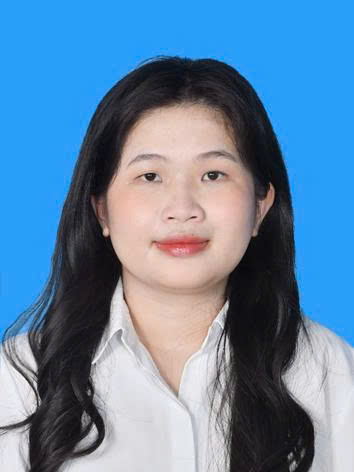
\includegraphics[
        width=2.1cm,
        height=2.5cm,
        keepaspectratio
    ]{assets/avt.jpg}
\end{minipage}

\end{tabularx}

\vspace{2pt}
\textcolor{rulecol}{\rule{\linewidth}{0.6pt}}

% ─── CAREER OBJECTIVE ─────────────────────────────────

\section*{Career Objective}

{\small
Final-year Information Technology student with a strong foundation in data structures \& algorithms, pursuing a Data Engineer role. Hands-on experience designing end-to-end data pipelines (source systems to target repositories) with Python, SQL, dbt, PostgreSQL, and Apache Airflow, plus event-based/streaming ingestion with Kafka, Python data-processing scripts, Power BI dashboards, and low-code workflows with Power Apps. Eager to learn Azure Databricks and PySpark while building reliable, high-quality, and scalable data solutions.
}

% ─── EDUCATION ────────────────────────────────────────

\section*{Education}

\entry
{University of Transport Ho Chi Minh City (UTH)}
{10/2022 -- 10/2026}
{Bachelor of Information Technology -- Completed coursework}

{\small
\begin{cvitems}
    \item GPA: \textbf{3.4 / 4.0}
    \item \textbf{Excellent Scholarship} -- Semester 1, 2025
    \item \textbf{Second Prize -- AI Track},
    UTH Student Scientific Research Conference 2025
\end{cvitems}
}

% ─── TECHNICAL SKILLS ─────────────────────────────────

\section*{Technical Skills}

{\small
\begin{tabularx}{\linewidth}{@{}lX@{}}

\textbf{Data Engineering}
&
ETL/ELT, Data Pipeline, Data Ingestion, Data Quality \& Consistency, Data Transformation, Workflow Automation \& Scheduling
\\[1pt]

\textbf{Programming}
&
Python, SQL, Pandas, NumPy, Data Structures \& Algorithms
\\[1pt]

\textbf{Databases}
&
PostgreSQL, SQL Server, MySQL, MongoDB, Firebase,
Supabase, Neon PostgreSQL
\\[1pt]

\textbf{Data Tools / BI}
&
dbt, Apache Airflow, Power BI
\\[1pt]

\textbf{Streaming \& Infrastructure}
&
Apache Kafka, RabbitMQ, MinIO (Data Lake), Docker
\\[1pt]

\textbf{Backend / API}
&
FastAPI, RESTful API, Node.js
\\[1pt]


\textbf{Tools}
&
Git, Postman, VS Code, Jira, Confluence

\end{tabularx}
}

% ─── WORK EXPERIENCE ──────────────────────────────────

\section*{Work Experience}

\entry
{Gotik Consulting -- Data Engineer}
{Python \textbar{} dbt \textbar{} PostgreSQL \textbar{} Airflow \textbar{} Power BI}
{03/2026 -- 05/2026}

{\small
\begin{cvitems}
    \item Designed and implemented an end-to-end data pipeline taking Odoo business data from source systems to Neon PostgreSQL, ensuring data quality and consistency through cleaning and validation at every stage.

    \item Wrote Python scripts and ETL pipelines to extract, clean, transform, and load data according to the needs of analysts and other engineers.

    \item Developed dbt models to turn raw data into structured, reusable analytical datasets, making transformation logic easier to maintain and extend.

    \item Automated hourly data workflows with Apache Airflow, including task scheduling, dependency management, and monitoring of ETL runs.

    \item Built Power BI dashboards to visualize operational and business metrics, delivering interactive reports that meet end-user requirements.

    \item Wrote SQL queries for aggregation, filtering, joins, and analytical reporting, providing reliable data sources for downstream dashboards.
\end{cvitems}
}
% ─── PROJECTS ─────────────────────────────────────────

\section*{Featured Data Projects}

\entry
{Delivery Driver -- Order Management \& Data Analytics System}
{Python \textbar{} PostgreSQL \textbar{} Kafka \textbar{} MinIO \textbar{} RFM \textbar{} Association Rule Mining}
{12/2025 -- 02/2026}

{\small

\begin{cvitems}
    \item Built an automated, event-based data pipeline with Kafka, a MinIO Data Lake, and a PostgreSQL Data Warehouse to ingest and process order data in real time.
    \item Applied RFM and Association Rule Mining (Python) to analyze customer orders and frequent pickup--delivery location pairs.
    \item Generated location-based insights to support recommendations for opening new post offices or service locations.
    \item GitHub: \href{https://github.com/LeKhang-cn22h/BE-delivery-driver}{BE-delivery-driver}
\end{cvitems}

}

\vspace{2pt}

\entry
{VehicleScan -- Smart Parking Data System}
{Python \textbar{} PostgreSQL \textbar{} Firebase \textbar{} ESP32 \textbar{} Kafka}
{03/2025 -- 03/2026}

{\small
\begin{cvitems}
    \item Designed streaming data workflows that ingest and process vehicle and IoT sensor data via Kafka.
    \item Integrated AI models, sensor, and application data into a pipeline for real-time parking management.
    \item Wrote Python processing scripts and managed PostgreSQL/Firebase storage for data collection and processing.
    \item GitHub: \href{https://github.com/LeKhang-cn22h/VehicleScanner.git}{VehicleScanner}
\end{cvitems}
}

% ─── ADDITIONAL INFORMATION ───────────────────────────

\section*{Additional Information}

{\small

\begin{tabularx}{\linewidth}{@{}lX@{}}

\textbf{English}
&
Technical document reading and basic professional communication

\\[1pt]

\textbf{Working Style}
&
Independent, proactive, detail-oriented; quick to learn and apply new technologies.

\\[1pt]

\textbf{Availability}
&
Available for full-time Data Engineer opportunities.

\end{tabularx}

}

\end{document}